% docs/images/b210_blockdiagram.tex -- receive path of the Ettus USRP B210 in Interferosim (TikZ, standalone)
% Version 0.1.0 (2026-10-31): first version
% Signal path of one station: antenna, external LNA, AD9361 (gain, quadrature
% mixer, low-pass filter, 12-bit ADC), FPGA (decimation, time stamps), USB 3.0,
% host (UHD, IQ recording). Reference: internal TCXO or GPSDO (10 MHz, PPS).
% Values: configs/receivers/b210.toml (data sheet) and b210_gpsdo.toml.
% Build:  pdflatex b210_blockdiagram.tex   -> b210_blockdiagram.pdf
% PNG (notebook 02):  pdftoppm -r 160 -png -singlefile b210_blockdiagram.pdf b210_blockdiagram
% ================================================================
\documentclass[tikz,border=4pt]{standalone}
\usepackage{amsmath}
\usetikzlibrary{arrows.meta,positioning,calc,fit,backgrounds,shapes.geometric}

\definecolor{chipbg}{RGB}{232,240,255}
\definecolor{boardbg}{RGB}{245,245,245}
\definecolor{refbg}{RGB}{255,246,214}
\definecolor{hostbg}{RGB}{226,245,226}

\begin{document}
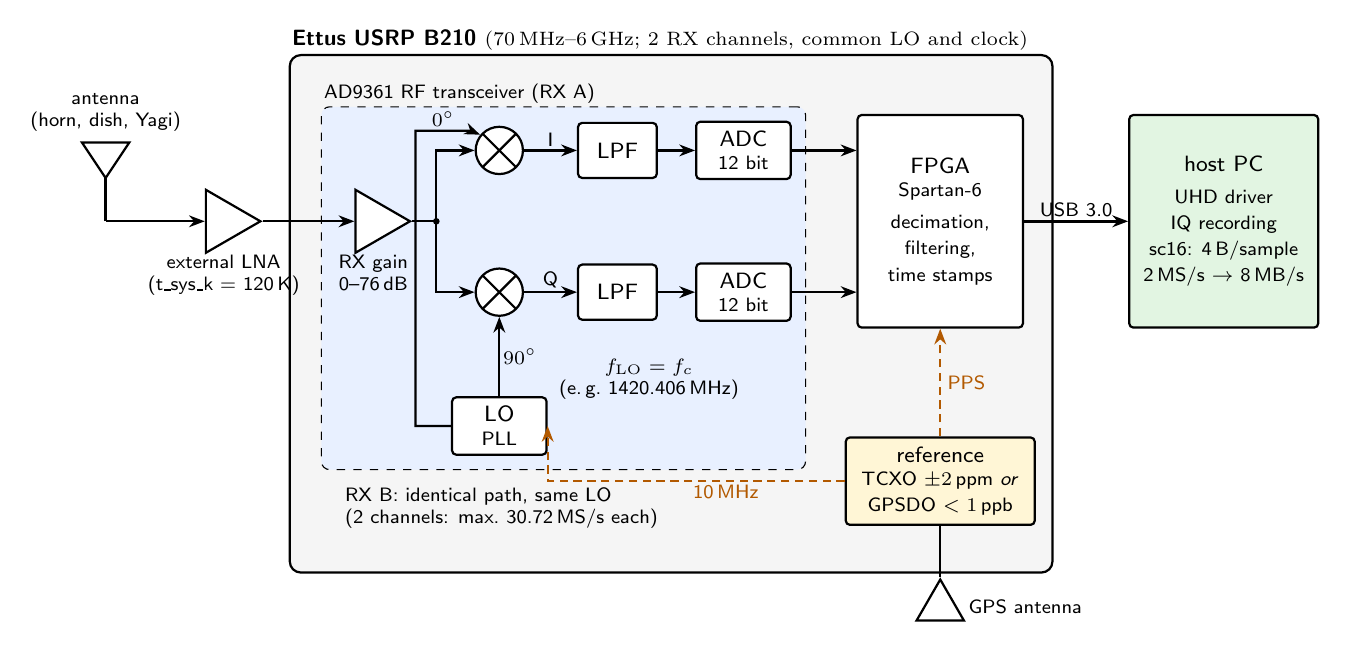
\begin{tikzpicture}[
    font=\sffamily\footnotesize,
    >={Stealth[length=2mm]},
    node distance=6mm and 7mm,
    blk/.style={draw, thick, fill=white, rounded corners=1.5pt, align=center,
                minimum height=9mm, minimum width=13mm},
    amp/.style={draw, thick, fill=white, isosceles triangle, isosceles triangle apex angle=60,
                minimum width=8mm, inner sep=0.5pt},
    mix/.style={draw, thick, fill=white, circle, minimum size=6mm, inner sep=0pt,
                path picture={\draw (path picture bounding box.north west) -- (path picture bounding box.south east)
                                    (path picture bounding box.north east) -- (path picture bounding box.south west);}},
    sig/.style={->, thick},
    ref/.style={->, thick, densely dashed, orange!70!black},
    lab/.style={font=\sffamily\scriptsize, inner sep=1pt},
  ]

  % ------------------------------------------------------------ antenna and external LNA
  \coordinate (ant) at (0,0);
  \draw[thick] (ant) -- ++(0,0.55);
  \draw[thick, fill=white] (ant)++(0,0.55) -- ++(-0.3,0.45) -- ++(0.6,0) -- cycle;
  \node[lab, above=11mm of ant, align=center] {antenna\\(horn, dish, Yagi)};
  \node[amp] (lna) at (1.5,0) {};
  \node[lab, below=1mm of lna, align=center] {external LNA\\(t\_sys\_k = 120\,K)};
  \draw[sig] (ant) -- (lna.west);

  % ------------------------------------------------------------ AD9361 receive path
  \node[amp] (gain) at (3.4,0) {};
  \node[lab, below=1mm of gain, align=center] (gainlab) {RX gain\\0--76\,dB};
  \coordinate (split) at (4.2,0);
  \node[mix] (mixI) at (5.0, 0.9) {};
  \node[mix] (mixQ) at (5.0,-0.9) {};
  \node[blk, minimum width=10mm, minimum height=7mm] (lpfI) at (6.5, 0.9) {LPF};
  \node[blk, minimum width=10mm, minimum height=7mm] (lpfQ) at (6.5,-0.9) {LPF};
  \node[blk, minimum width=12mm, minimum height=7mm] (adcI) at (8.1, 0.9) {ADC\\[-1pt]\scriptsize 12 bit};
  \node[blk, minimum width=12mm, minimum height=7mm] (adcQ) at (8.1,-0.9) {ADC\\[-1pt]\scriptsize 12 bit};
  \node[blk, minimum width=12mm, minimum height=7mm] (lo) at (5.0,-2.6) {LO\\[-1pt]\scriptsize PLL};
  \draw[sig] (lna.east) -- (gain.west);
  \draw[thick] (gain.east) -- (split);
  \fill (split) circle (1.2pt);
  \draw[sig] (split) |- (mixI.west);
  \draw[sig] (split) |- (mixQ.west);
  \draw[sig] (mixI) -- node[lab, above]{I} (lpfI);
  \draw[sig] (mixQ) -- node[lab, above]{Q} (lpfQ);
  \draw[sig] (lpfI) -- (adcI);
  \draw[sig] (lpfQ) -- (adcQ);
  % LO with 0 / 90 degree outputs
  \draw[sig] (lo.north) -- node[lab, right]{$90^\circ$} (mixQ.south);
  \draw[sig] (lo.west) -- ++(-0.45,0) |- node[lab, pos=0.75, above]{$0^\circ$} ($(mixI.west)+(-0.05,0.25)$) -- ++(0.12,-0.05);
  \node[lab, align=center] at (6.9,-2.0) {$f_\mathrm{LO} = f_c$\\(e.\,g.\ 1420.406\,MHz)};

  % ------------------------------------------------------------ FPGA, USB, host
  \node[blk, minimum width=21mm, minimum height=27mm] (fpga) at (10.6,0)
    {FPGA\\[-1pt]\scriptsize Spartan-6\\[2pt]\scriptsize decimation,\\\scriptsize filtering,\\\scriptsize time stamps};
  \draw[sig] (adcI.east) -- (adcI.east -| fpga.west);
  \draw[sig] (adcQ.east) -- (adcQ.east -| fpga.west);

  \node[blk, fill=hostbg, minimum width=24mm, minimum height=27mm] (host) at (14.2,0)
    {host PC\\[2pt]\scriptsize UHD driver\\\scriptsize IQ recording\\\scriptsize sc16: 4\,B/sample\\\scriptsize 2\,MS/s $\to$ 8\,MB/s};
  \draw[sig, line width=1.2pt] (fpga) -- node[lab, above]{USB 3.0} (host);

  % ------------------------------------------------------------ reference: TCXO or GPSDO
  \node[blk, fill=refbg, minimum width=24mm] (refclk) at (10.6,-3.3)
    {reference\\[-1pt]\scriptsize TCXO $\pm 2$\,ppm  \emph{or}\\\scriptsize GPSDO $< 1$\,ppb};
  \node[amp, shape border rotate=90, minimum width=6mm] (gps) at (10.6,-4.9) {};
  \draw[thick] (gps.apex) -- (refclk.south);
  \node[lab, right=1mm of gps] {GPS antenna};
  \draw[ref] (refclk.west) -- node[lab, below, pos=0.4]{10\,MHz} (lo.east |- refclk.west) -- (lo.east);
  \draw[ref] (refclk.north) -- (fpga.south);
  \node[lab, orange!70!black, anchor=west] at ($(fpga.south)!0.5!(refclk.north)+(0.05,0)$) {PPS};

  % ------------------------------------------------------------ frames
  \node[lab, align=left, anchor=north west] (rxb) at (3.0,-3.35)
    {RX B: identical path, same LO\\(2 channels: max.\ 30.72\,MS/s each)};
  \begin{scope}[on background layer]
    \coordinate (boardtop) at (2.55,1.9);
    \coordinate (boardbot) at (3.0,-4.25);
    \node[draw, thick, fill=boardbg, rounded corners=4pt, inner sep=6pt,
          fit=(gain)(gainlab)(fpga)(refclk)(rxb)(boardtop)(boardbot)] (board) {};
    \node[draw, dashed, fill=chipbg, rounded corners=3pt, inner sep=5pt,
          fit=(gain)(gainlab)(mixI)(mixQ)(lpfI)(adcI)(adcQ)(lo)] (chip) {};
  \end{scope}
  \node[lab, anchor=south west] at (chip.north west) {AD9361 RF transceiver (RX A)};
  \node[lab, anchor=south west, font=\sffamily\footnotesize\bfseries] at (board.north west)
    {Ettus USRP B210 \normalfont\scriptsize(70\,MHz--6\,GHz; 2 RX channels, common LO and clock)};
\end{tikzpicture}
\end{document}
